\section{Diverses}
\subsection{Zahlencodes}
\begin{center}
    \csvreader[
        separator=semicolon,
        tabular=|c|cccccc|,
        head=true,
        table head=\hline\rotatebox{90}{Binär} & \rotatebox{90}{BCD} & \rotatebox{90}{Excess-3~} & \rotatebox{90}{Aiken} & \rotatebox{90}{4-2-2-1} & \rotatebox{90}{Gray} & \rotatebox{90}{O'Brien}\\\hline,
        table foot = \hline,
        late after line=\csvifoddrow{\\\rowcolor{white}}{\\\rowcolor{primaryheader!15}}
        ]{tables/codes.csv}{
            1=\binary, 
            2=\bcd, 
            3=\excessThree, 
            4=\aiken, 
            5=\ftto, 
            6=\gray, 
            7=\obrien
            }{%
            \binary & \bcd & \excessThree & \aiken & \ftto & \gray & \obrien
    }%
\end{center}

\subsection{Gate Varianten}
\begin{center}
    \rotatebox{90}{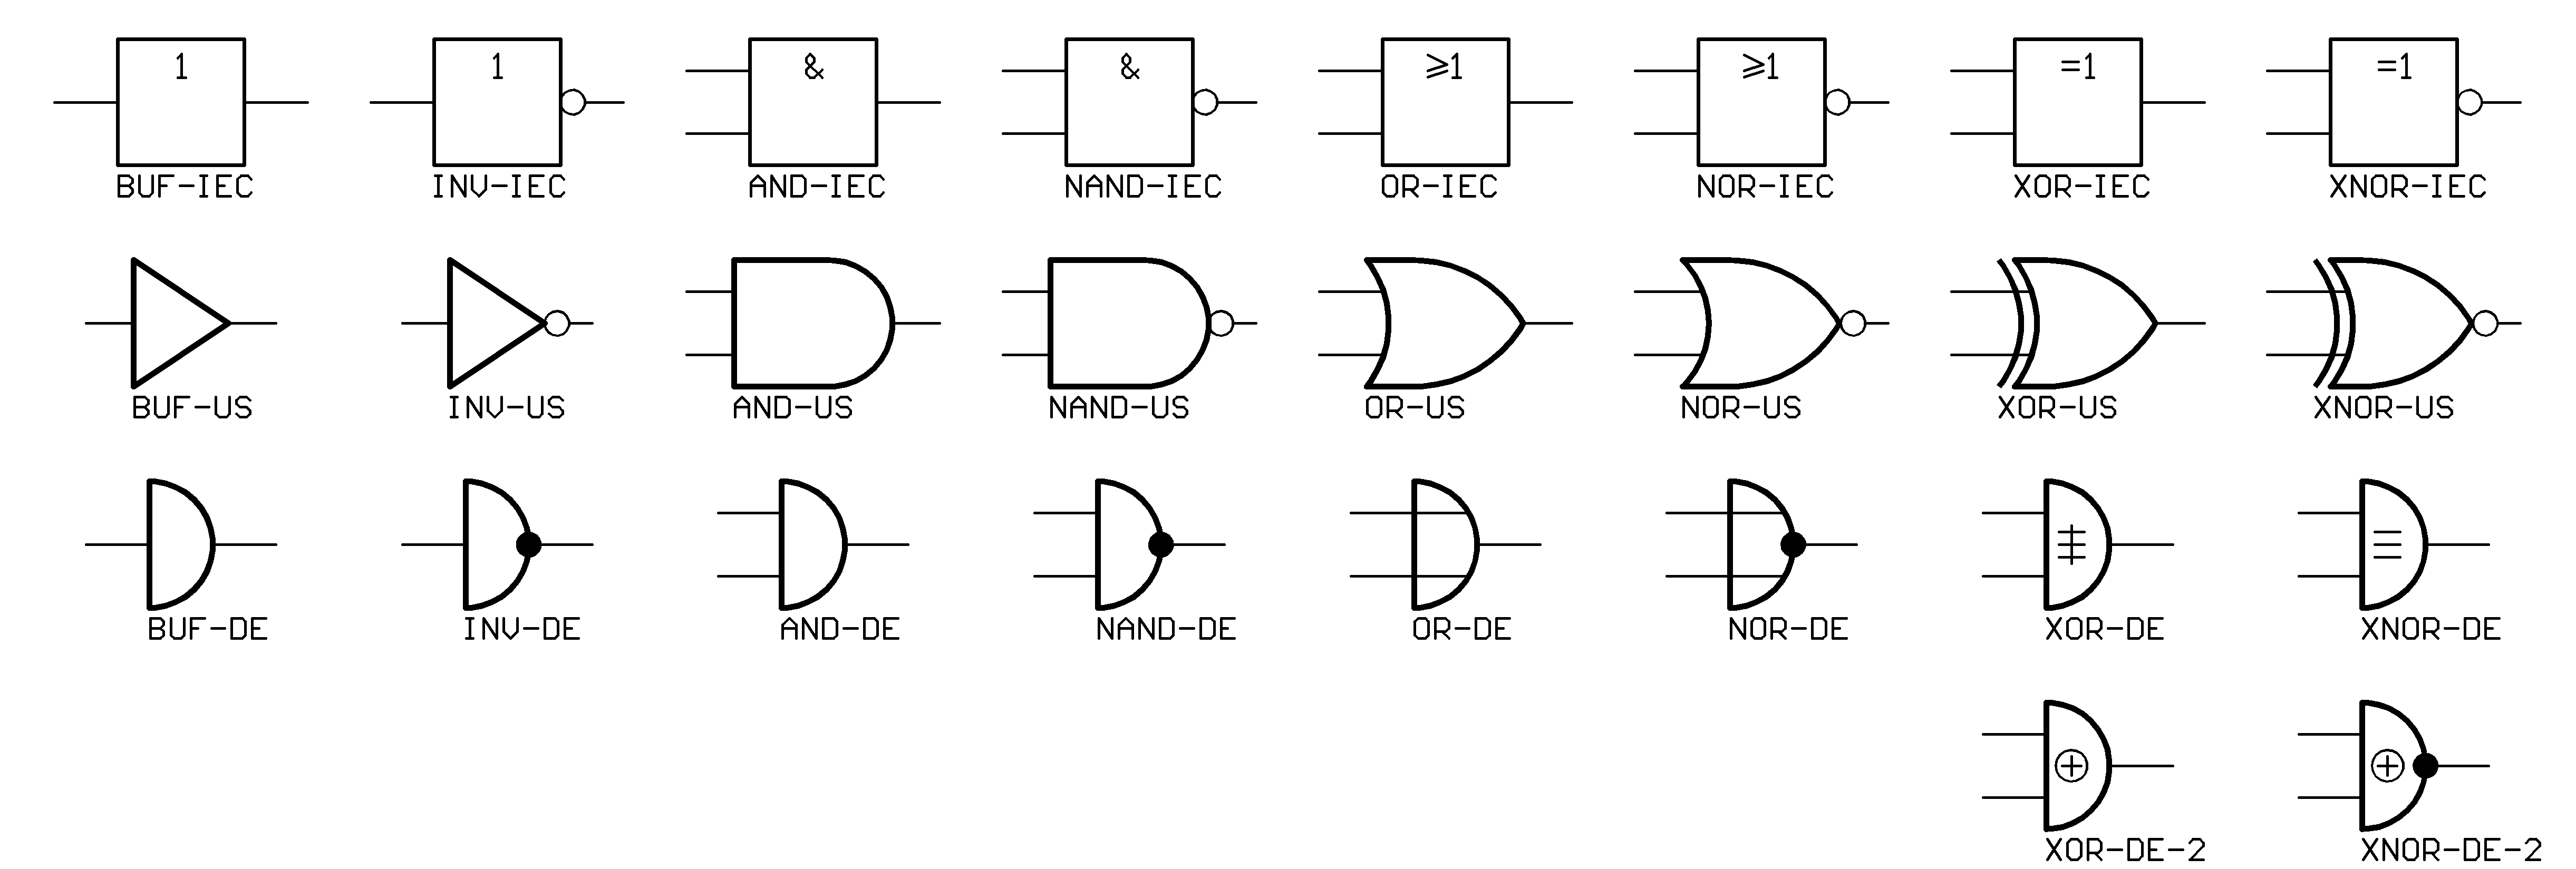
\includegraphics[width = 120mm]{images/Logic-gate-index.png}}
\end{center}

\subsection{Zehnerpotenzen}
\begin{center}
    \renewcommand{\arraystretch}{1.25}
    \rowcolors{2}{primaryheader!15}{white}
    \begin{tabular}{|clc|}
        \hline
        \rowcolor{white}
        Potenz & Präfix & Symbol\\
        \hline
        $10^{-15}$   &   Femto   &   f       \\
        $10^{-12}$   &   Piko    &   p       \\
        $10^{-9}$    &   Nano    &   n       \\
        $10^{-6}$    &   Mikro   &   $\mu$   \\
        $10^{-3}$    &   Milli   &   m       \\
        $10^{-2}$    &   Zenti   &   c       \\
        $10^{-1}$    &   Dezi    &   d       \\
        \hline
        $10^1$     &   Deka    &   da      \\
        $10^2$     &   Hekto   &   h       \\
        $10^3$     &   Kilo    &   k       \\
        $10^6$     &   Mega    &   M       \\
        $10^9$     &   Giga    &   G       \\
        $10^{12}$  &   Tera    &   T       \\
        $10^{15}$  &   Peta    &   P       \\
        \hline
    \end{tabular}
\end{center}

\subsection{Erweiterte Zweierpotenzen}
\begin{center}
    \rowcolors{2}{primaryheader!15}{white}
    \begin{tabular}{|cr||cl|}
        \hline
        \rowcolor{primaryheader!15}$2^{0}$ & $1.0$ & $2^{-0}$ & $ 1.0$ \\ 
        $2^{1}$ & $2.0$ & $2^{-1}$ & $ 0.5$ \\ 
        $2^{2}$ & $4.0$ & $2^{-2}$ & $ 0.25$ \\ 
        $2^{3}$ & $8.0$ & $2^{-3}$ & $ 0.125$ \\ 
        $2^{4}$ & $16.0$ & $2^{-4}$ & $ 0.0625$ \\ 
        $2^{5}$ & $32.0$ & $2^{-5}$ & $ 0.03125$ \\ 
        $2^{6}$ & $64.0$ & $2^{-6}$ & $ 0.015625$ \\ 
        $2^{7}$ & $128.0$ & $2^{-7}$ & $ 0.0078125$ \\ 
        $2^{8}$ & $256.0$ & $2^{-8}$ & $ 0.00390625$ \\ 
        $2^{9}$ & $512.0$ & $2^{-9}$ & $ 0.001953125$ \\ 
        $2^{10}$ & $1024.0$ & $2^{-10}$ & $ 9.765625^{-4}$ \\ 
        $2^{11}$ & $2048.0$ & $2^{-11}$ & $ 4.8828125^{-4}$ \\ 
        $2^{12}$ & $4096.0$ & $2^{-12}$ & $ 2.44140625^{-4}$ \\ 
        \hline                
    \end{tabular}
\end{center}
